%======================================================================
\subsection{BW-UIX-04 --- Built, 26 Oct: the history timeline}\label{sec:uix04-built}
%======================================================================

The spike's bottom bar (\#7) is now the full Fusion-style timeline, built in six commits on 26 Oct
(\code{a60365c}, \code{c078b20}, \code{d10f603}, \code{46f6d0b}, \code{a38c56d}, \code{41998ab}), all Python in
\file{package/bruceworx/mods/HistoryTimeline/}. Your earlier decisions were kept as they stand
(\S\ref{sec:ui-design}: one row, no dock title, 20\,px chips in theme colours, rolled-back items dimmed, hidden
without history, creation order and no playback or marker for assemblies, the active body wins).

\begin{figure}[!htbp]
\centering
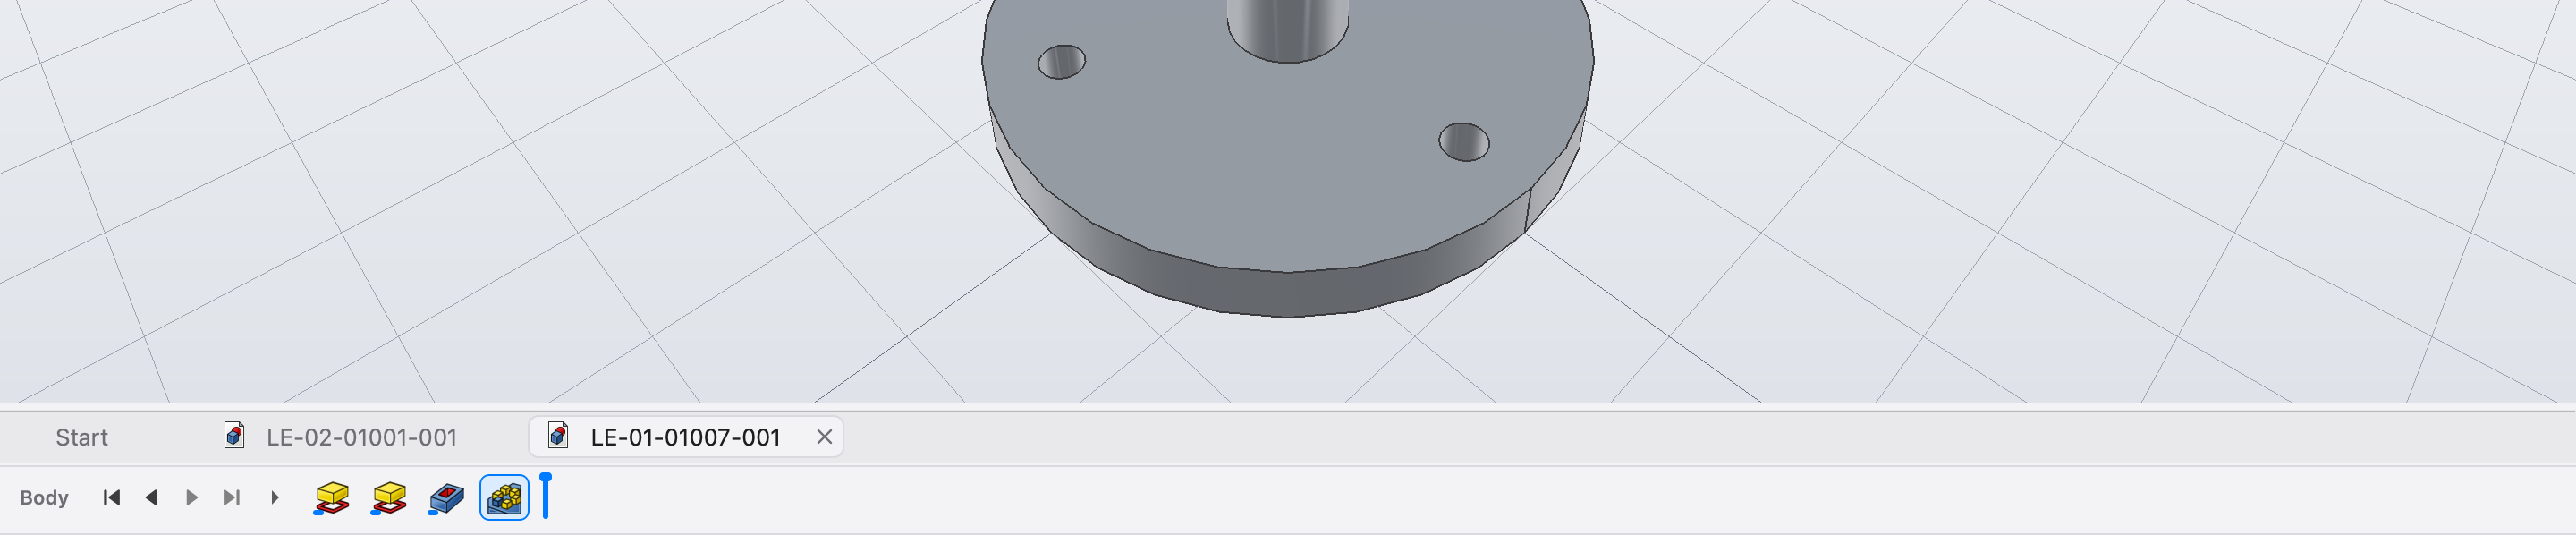
\includegraphics[width=\linewidth]{fig/uix04_timeline_light.png}\\[3pt]
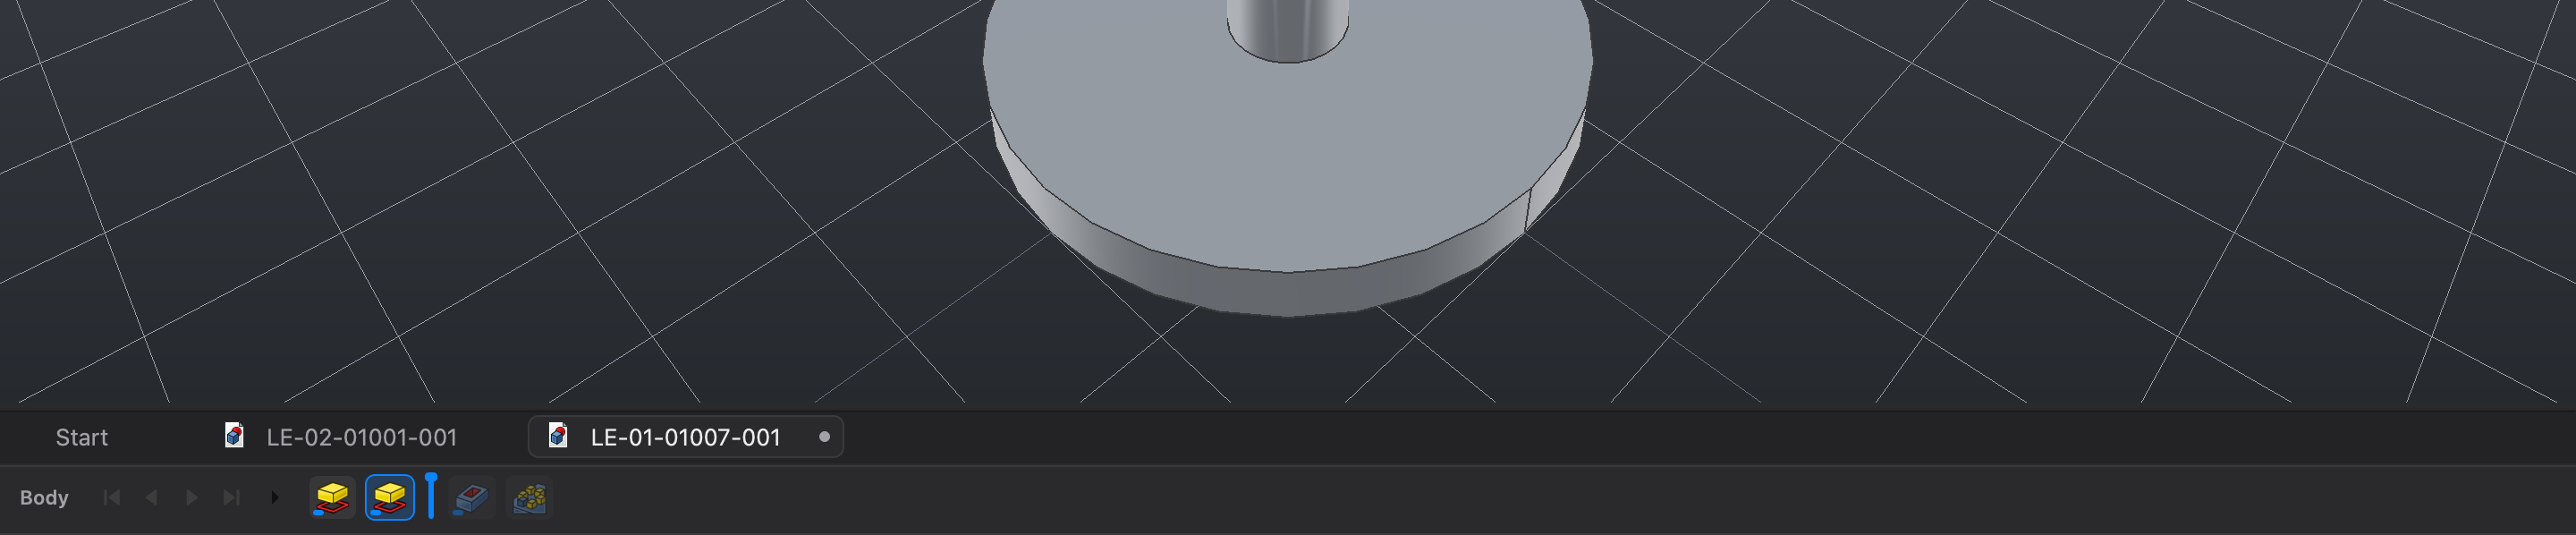
\includegraphics[width=\linewidth]{fig/uix04_rolled_dark.png}
\caption{The planet carrier \code{LE-01-01007-001} (a copy, with its parameter sheet open) in the timeline. Top,
light: the whole history in one row, playback buttons, the disclosure for the folded sketches, the marker after
the pattern. Bottom, dark: the marker dragged back to the shaft pad; the pin hole and its pattern are dimmed and
the 3D view shows the disc and shaft only.}
\label{fig:uix04-built}
\end{figure}

\paragraph{What you can do on the bar now.}
\begin{itemize}[nosep]
  \item \textbf{Drag the marker.} It rolls the body back and forward as it crosses the chips: each crossing sets
        \code{Body.Tip}, shows only that feature and recomputes, so the 3D view follows the hand. One undo step
        per drag (``Roll history tip''); Escape puts everything back; dropping where it was adds no step. A body
        with more than 40 Group entries keeps the marker and the dimming live but sets the tip once, at the drop.
  \item \textbf{Playback}: to start, back one, forward one, to end, at the left of the bar, with their own light
        and dark SVGs in the mod. ``To start'' clears the tip, as Fusion's first button does. Hidden for assemblies.
  \item \textbf{Right-click}: Edit feature, Rename (inline, over the chip), Suppress / Unsuppress, Roll history
        to here, Delete, Move earlier, Move later. Delete goes through \code{Std\_Delete}, so FreeCAD's own
        ``Object dependencies'' question appears when later features depend on it.
  \item \textbf{Reorder.} Move earlier / later swap a feature with its neighbour through the same App calls as
        \code{PartDesign\_MoveFeatureInTree} (\code{Body.removeObject} + \code{insertObject}), and the feature's own
        sketch travels with it. The action is enabled only when the move is legal; a disabled action's tooltip says
        why (``Pins $\times$ n\_planets uses Pin hole \O3, which would come after it'', ``Pin hole \O3 needs material
        before it; it cannot be the first feature'').
  \item \textbf{Chips}: a red badge on a feature that failed to recompute (its tooltip carries FreeCAD's error),
        hovering preselects the feature in the 3D view and the tree, tooltips say \emph{Label / Kind $\cdot$ Name /
        on Base / state}. A sketch used by one feature is folded under it (small mark on the chip); the disclosure
        at the left opens them, and the choice is remembered.
\end{itemize}

\begin{figure}[!htbp]
\centering
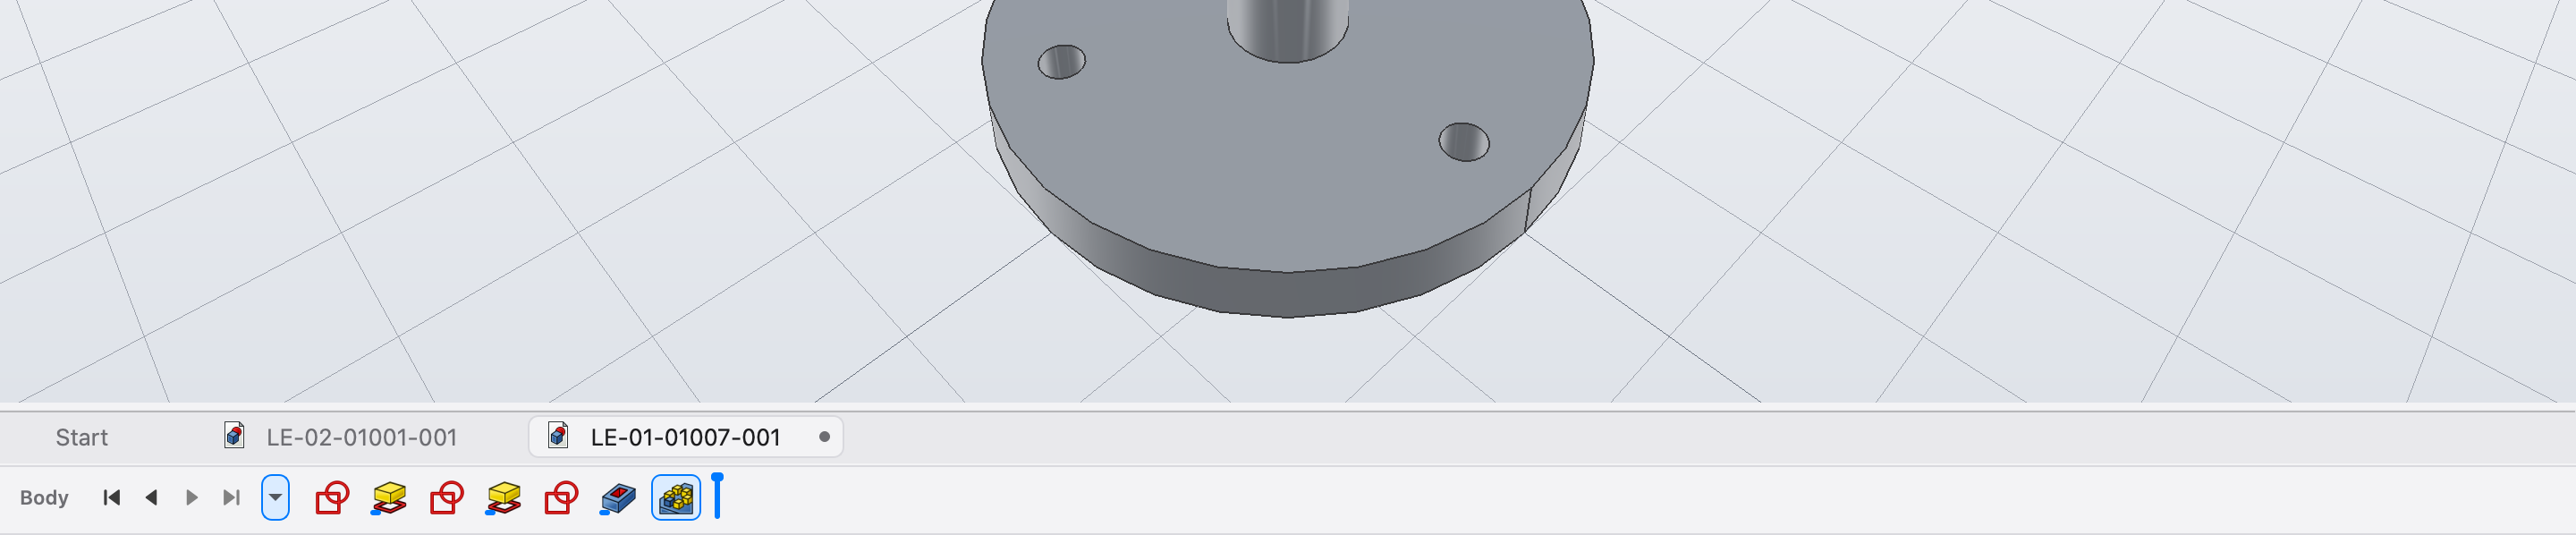
\includegraphics[width=0.74\linewidth]{fig/uix04_expanded_light.png}\hfill
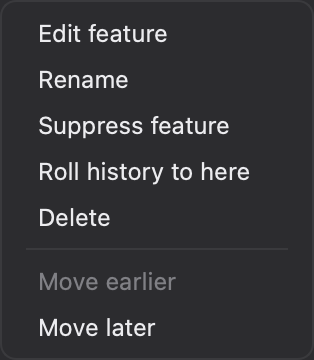
\includegraphics[width=0.24\linewidth]{fig/uix04_menu_dark.png}
\caption{Left: the disclosure opened, each sketch beside its feature. Right: the chip menu (dark).}
\label{fig:uix04-menu}
\end{figure}

\paragraph{Decided while building.}
\begin{itemize}[nosep]
  \item \textbf{The marker stays \code{Body.Tip}.} Features after it still recompute; the file stays readable by
        stock FreeCAD. A Fusion-style ``do not compute'' state would be a body property and is left for core
        (\file{docs/CORE.md}).
  \item \textbf{Legal reorder = no link crosses the wrong way.} A move is refused when any member of the group
        that ends up earlier links (any property except the solid chain) a member of the group it crosses, or when a
        subtractive feature, dress-up or pattern would become the first solid. \code{isFeatureMovable} in
        PartDesign answers a different question (can the feature leave the body) and was not used.
  \item \textbf{Dress-ups are rebound by geometry.} Found while building: after the body relinks a fillet, its
        mapped element names (\code{;\#18:1;:H3b1,E.Edge1}) still describe the old base and the fillet reports
        ``Invalid edge link''. Before a move the timeline notes each referenced edge or face (type, size, centre);
        after the first recompute it finds the same geometry on the new base and writes plain names, which FreeCAD
        maps afresh. If an element no longer exists the move is undone in the Report view (``move of Fillet
        undone, \ldots''). The acceptance moved a fillet before an independent through hole and back with the same
        volume.
  \item \textbf{The tip stays on its object} after a move, except that a tip at the end stays at the end.
  \item \textbf{Playback steps over suppressed solids} (the marker may rest after them), as the spike's rule that
        suppression and the tip are different things.
  \item \textbf{Hover highlight is preselection}, not selection, so a hover never changes what a command acts on.
  \item \textbf{Old chips are detached at once.} \code{deleteLater} alone left the previous chips painting until
        the event loop came back (ghosts in scripted grabs and in nested loops).
\end{itemize}

\paragraph{Tests.} Headless (\file{tests/test\_timeline\_access.py}): 141 checks, among them playback, delete,
every legal and illegal reorder rule, the fillet before and after the hole, a sketch travelling with its pocket,
fold and error entries; the assembly suite's 31 pass unchanged. GUI (\file{src/Mod/BruceWorx/TestBruceWorxTimeline.py},
under \file{run\_gui\_tests.py}): 25 tests with synthetic mouse events on the bar: drag back, forward, to the front,
Escape, same-place drop, live preview and the big-body drop; playback; the menu (rename, delete with and without
the dependency dialog, roll, suppress); reorder with undo and the disabled illegal moves; badge, hover, tooltips,
folding. Acceptance (\file{SCRATCH/agent-uix04/accept/}): on a copy of the carrier, 23 steps pass in light and in
dark with no Report errors: the row, the drags, playback, the pin hole moved before the output shaft with the same
volume and its sketch along, the pattern's and the disc's illegal moves disabled, undo.

\paragraph{Path into core.} \file{docs/CORE.md} in the mod: a \code{Gui::HistoryTimeline} dock with a provider
interface per module, the PartDesign provider taking over \code{isSolidFeature} / \code{isMultiTransformChild} and
the dress-up rebind (which belongs next to \code{DressUp::onChanged}), icons in \file{src/Gui/Icons}; the menu item,
pick trace and headless tests stay Python; preference keys \code{Mod/HistoryTimeline/Enabled},
\code{HideWhenEmpty}, \code{ShowSketches}.

\paragraph{Open questions for you.}
\begin{enumerate}[nosep]
  \item \textbf{Rolled-back features still compute.} Keep \code{Tip} (file compatibility) or add a real rolled-back
        state in core later? The bar is honest either way (dimmed means ``after the marker'').
  \item \textbf{Sketches folded by default.} The disclosure is closed on first start (\code{ShowSketches} false),
        as Fusion. Prefer them open?
  \item \textbf{``To start'' clears the tip} and leaves an empty body on screen, as Fusion. Prefer it to stop at the
        first feature?
  \item \textbf{Reorder of a feature whose sketch sits on another feature's face} is refused rather than offered
        with a warning. Fusion refuses too; say if you want the warning-and-try variant.
  \item \textbf{The GUI module flaked once}: two runs out of nine lost the synthetic marker press (every drag test),
        then passed unchanged with diagnostics in place and in all later runs. Suspect: the test window being moved by
        the placement helper mid-test. Not reproduced; left as is.
\end{enumerate}
